\documentclass[11pt,letterpaper]{article}

\input{../../../../.config/latex/preamble_v1.tex}

\lightmode

\title{\textbf{Math 231a Problem Set 1}}

\begin{document}
\maketitle

\begin{problem}
    Let $\Delta$ be the category of totally ordered finite sets with weakly order preserving maps, and let $\Delta_{\text{inj}}$ be the subcategory of $\Delta$ with injective order preserving maps. Show the following equivalences of categories: 
    \begin{enumerate}
        \item $\mathbf{sSet} \cong \textrm{Fun}(\Delta^{\text{op}}, \mathbf{Set})$. 
        \item $\mathbf{ssSet} \cong \textrm{Fun}(\Delta_{\text{inj}}^{\text{op}}, \mathbf{Set})$. 
    \end{enumerate}
\end{problem}

\begin{solution}
    Recall that a simplicial set is a sequence of sets $\{K_i\}_{i\geq 0}$ with face/degeneracy maps $s_i, d_j$. Given some contravariant functor $F : \Delta \to \mathbf{Set}$, consider the simplicial set $\{F([i])\}_{i=0}$ with face/degeneracy maps $F(d_i)$ and $F(s_i)$, where $d_i$ is the order preserving map skipping $i$ and $s_i$ is the order preserving map doubling up on $i$. Note that contravariance sends $d_i : [n] \to [n+1]$ to $F(d_i) : K_{n+1} \to K_n$ and similarly for $s_i$. Since $F$ preserves composition, Problem~1 on Problem Set~1 shows that the maps $F(d_i)$ and $F(s_i)$ follow the axioms of a simplicial set. So $\textrm{Fun}(\Delta^\text{op}, \mathbf{Set}) \subset \mathbf{sSet}$. Natural transformations of two functors $F, D: \Delta \to \mathbf{Set}$. Correspond to maps of simplicial sets in the following way: For each $i$, consider the map $F([i]) \to D([i])$ given by the natural transformation. This is a simplicial set basically by definition.
    
    Conversely, given a simplicial set $\{K_i\}_{i\geq 0}$, we can consider the contravariant functor $F : \Delta \to \mathbf{Set}$ which sends $[n]$ to $K_n$, sends the face and degeneracy maps to $d_i$ and $s_i$ respectively. Since every order preserving map factors uniquely as a composition of a $d_i$ and an $s_i$, this fully defines a set map for every order preserving map $[n] \to [m]$. Again, the identities are preserved on both sides, so this gives us a unique functor. Thus $\mathbf{sSet} \cong \textrm{Fun}(\Delta^{\text{op}}, \mathbf{Set})$.  

    The same thing happens for $\mathbf{ssSet}\cong \text{Fun}(\Delta^{\text{op}}_{\text{inj}}, \mathbf{Set})$.  
\end{solution}

\begin{problem}
    Let $\pi_0(X)$ denote the set of path components of a space $X$. Prove that there is a natural isomorphism $\Z\pi_0(X) \isom H_0(X)$.
\end{problem}

\begin{solution}
    For any space $X$, lets define the map $\phi_X : \Z\pi_0(X) \to H_0(X)$ by sending any path component $X_i$ to $[c_{x_i}^0]$ for any $x_i\in X_i$. Clearly this is well defined, since if $y_i\in X_i$ is any other point in the same path component, with $\gamma : \Delta^1 \to X_i$ a path connecting them, them $d\gamma = c_{x_i}^0 - c_{y_i}^0$ in $H_0(X)$ and so $[c_{x_i}^0]=[c_{y_i}^0]$ in $H_0(X)$. We can define the map on all of $\Z\pi_0(X)$ by extending linearly in the natural way. This map is clearly injective since $\Delta^1$ is connected, and surjective because the inverse image of any $c_{x}^0$ is the path component of $X$.

    Now suppose $f : X \to Y$ is a continuous map. We have a natural induced map $\Z\pi_0(f) : \Z\pi_0(X) \to \Z\pi_0(Y)$, which sends the path component of $x$ to the path component of $f(x)$. To prove naturality, notice that $H_0(f)(\phi_X(x))=H_0(f)([c_x^0])=[f\circ c_x^0]=[c_{f(x)}^0]$. On the other side, we have $\phi_Y(\Z\pi_0(f)(x))=\phi_Y(f(x))=[c_{f(x)}^0]$. This means that extended linearly, the maps must be equal and so the transformation is natural.
\end{solution}

\begin{problem}
    Let $X$ be a path-connected space and let $x\in X$. We will show a natural isomorphism
    \[
        \pi_1(X,x)^{\text{ab}} \isom H_1(X)
    .\] 
    Given a path $f :I\cong \Delta^1 \to X$, let $[f]\in S_1(X)$ denote the corresponding singular 1-chain.
    \begin{enumerate}[(a)]
        \item Let $f,g : I \to X$ denote two paths with $f(0)=g(0)$ and $f(1)=g(1)$. Suppose that $f\simeq g$ rel $\partial I$, i.e. there is a homotopy $h: I\times I\to X$ between $f$ and $g$ which is constant on $\{0\}\times I$ and $\{1\}\times I$. Prove that $[f]\equiv [g]\mod B_1(X)$.
        \item Given two paths $f,g$ such that $f(1)=g(0)$, prove that $[f*g]\equiv [f]+[g]\mod B_1(X)$, where $f*g$ is the composition of $f$ and $g$. Conclude that there is a group homomorphism 
        \[
            \phi_* : \pi_1(X,x)^\text{ab} \to H_1(X)    
        \]
        sending the homotopy class of a loop $f$ to $[f]$.
        \item For each point $y\in X$, fix a path $\lambda_y$ from $x$ to $y$. Define a map 
        \[
            \psi : S_1(X) \to \pi_1(x,x)^\text{ab}    
        \]
        by sending $[f]$ to the image of the homotopy class of $\lambda_{f(0)}*f*\overline{\lambda_{f(1)}}$ in the abelianization. Here, $\overline{\lambda_{f(1)}}$ is the reverse of the path $\lambda_{f(1)}$. Prove that $\psi$ sends all elements of $B_1(X)$ to the identity element, so that $\psi$ induces a map: \[
            \psi_* : H_1(X) \to \pi_1(X,x)^\text{ab}
        .\]
        \item Prove that $\psi_* \circ \phi_* = \text{id}_{\pi_1(X,x)^\text{ab}}$ and $\phi_* \circ \psi_* = \id_{H_1(X)}$, so that $\phi_*$ and $\psi_*$ are inverse isomorphisms.  
    \end{enumerate}
\end{problem}

\begin{solution}
    \textbf{(a)} Let $v_0=f(0)$ and $v_1=f(1)$. Consider the simplex $\sigma \in S_2(h(I\times I))$ given by the triangulation
    \begin{center}
        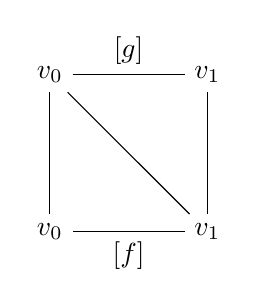
\begin{tikzpicture}
            \node[] (A) at (-1,-1) {$v_0$};
            \node[] (B) at (-1,1) {$v_0$};
            \node[] (C) at (1,-1) {$v_1$};
            \node[] (D) at (1,1) {$v_1$};
            \draw[] (C) -- node[below] {$[f]$} (A);
            \draw[] (A) -- (B);
            \draw[] (B) -- node[above] {$[g]$} (D);
            \draw[] (D) -- (C);
            \draw[] (B) -- node[above] {} (C);
        \end{tikzpicture}
    \end{center}

    Then $d\sigma = [f] - [g] + c_{v_0}^1 + c_{v_1}^1$. But note that any $1$-simplex is a boundary because $d c_x^2 = c_x^1 - c_x^1 + c_x^1 = c_x^1$. This means that $0\equiv d\sigma \equiv [f]-[g]+c_{v_0}^1+c_{v_1}^1\equiv [f]-[g]\mod B_1(X)$ and so $[f]\equiv [g]\mod B_1(X)$ as desired.

    \textbf{(b)} Consider the simplex $\sigma \in S_2(X)$ given by
    \begin{center}
        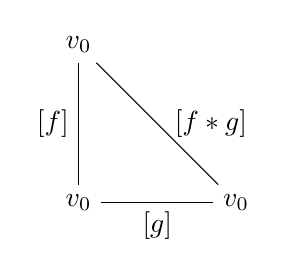
\begin{tikzpicture}
            \node[] (0) at (-1, -1) {$v_0$};
            \node[] (1) at (-1,1) {$v_0$};
            \node[] (2) at (1,-1) {$v_0$};
            \draw[] (0) -- node[left] {$[f]$} (1);
            \draw[] (1) -- node[right] {$\;[f*g]$} (2);
            \draw[] (2) -- node[below] {$[g]$} (0);
        \end{tikzpicture}
    \end{center}
    More explicitly, the map can be given by
    \[
        \sigma(x,y) = \begin{cases}
            f(x+y) & x < y\\
            g(x+y) & x \geq y
        \end{cases}
    .\] 
    This map is clearly continuous, and in particular note that $\sigma(0,t)=f(t)$, $\sigma(t,0)=g(t)$, and $\sigma(t, (1-t))=(f*g)(t)$, as shown in the diagram. So $d\sigma = [f]-[f*g]+[g]$ and so $[f*g]\equiv [f]+[g]\mod B_1(X)$. Thus, we have a well defined map $\phi_*$ from $\pi_1(X,x)^\text{ab} \to H_1(X)$ since every loop $f*g*\overline{f}*\overline{g}\in [\pi_1(X,x), \pi_1(X,x)]$ maps to $[f]+[g]-[f]-[g]=0$.  

    \textbf{(c)} Let $\sigma : \Delta^2 \to X$ be a $2$-simplex with vertices $x_0, x_1, x_2 \in X$ and edges $e_0, e_1, e_2 : \Delta^1 \to X$ respectively. Then
    \[
        \begin{aligned}
            \psi(d\sigma) = \psi(e_0 - \overline{e_1} + e_2) &= \psi(e_0 + e_2 - \overline{e_1}) = \psi(e_0) * \psi(e_2) * \overline{\psi(\overline{e_1})}\\
            &=[\lambda_{x_0} * e_0 * \overline{\lambda_{x_1}}] * [\lambda_{x_1} * e_2 * \overline{\lambda_{x_2}}] * \overline{[\lambda_{x_0} * \overline{e_1} * \overline{\lambda_{x_2}}]}\\
            &=[\lambda_{x_0} * e_0 * \overline{\lambda_{x_1}} * \lambda_{x_1} * e_2 * \overline{\lambda_{x_2}} * \lambda_{x_2} * e_1 * \overline{\lambda_{x_0}}]\\
            &=[\lambda_{x_0} * e_0 * e_2 * e_1 * \overline{\lambda_{x_0}}].
        \end{aligned}
    \]  
    Since $e_0 * e_2 * e_1$ is homotopic to a constant map, this is zero, so $\psi$ sends $B_1(X)$to the identity class. This gives us our induced map.

    \textbf{(d)} For any loop $f\in \pi_1(X,x)$, we have $(\psi_*\circ \phi_*)(f) = [\lambda_{f(0)}*f*\overline{\lambda_{f(1)}}] \equiv [f]\mod [\pi_1(X,x), \pi_1(X,x)]$ and so $\psi_*\circ \phi_* = \text{id}_{\pi_1(X,x)^\text{ab}}$. Conversely for any 1-simplex $f\in H_1(X)$, we have $(\phi_*\circ\psi_*)(f)=\lambda_{f(0)}+f-\lambda_{f(1)}=f$ so we are done.  
\end{solution}

\begin{problem}
    Let $A_*$ be a chain complex. It is \emph{acyclic} if $H_*(A_*)=0$, and \emph{contractible} if it is chain-homotopy-equivalent to the trivial chain complex. 
    \begin{enumerate}[(a)]
        \item Prove that a chain complex is contractible if and only if it is acyclic and the inclusion $Z_*(A_*)\to A_*$ is a split monomorphism.
        \item Give an example of an acyclic chain complex that is not contractible. 
    \end{enumerate}
\end{problem}

\begin{solution}
    \textbf{(a)} Suppose first that $A_*$ is a contractible chain complex; i.e. there is a chain homotopy $h : A_* \to A_*$ between $0$ and $\text{id}$. This means $h$ satisfies $dh+hd=\text{id}$. Since chain homotopy equivalence preserves homology, it's clear that $A_*$ is acyclic, since it is chain homotopy equivalent to a trivial chain complex, which has trivial homology groups. To prove that $Z_*(A_*) \to A_*$ is a split monomorphism, note that we have a map $f : A_* \to Z_*(A_*)$ which sends $a$ to $dh(a)=a-hd(a)$. This is clearly a homomorphism, and we have
    \[
        Z_*(A_*) \longrightarrow A_* \longrightarrow Z_*(A_*)
    .\]   
    Observe that for any cycle $\sigma$, $f(\sigma)=dh(\sigma)=\sigma-hd(\sigma)=\sigma$, so $f$ is a left inverse to the inclusion and we are done. Now conversely suppose that $A_*$ is acyclic and $f : A_* \to Z_*(A_*)$ is a left inverse to the inclusion $Z_*(A_*) \to A_*$. We'll construct a chain homotopy to the trivial chain as follows: for any chain $\sigma\in A_*$, $f(\sigma)\in Z_*(A_*)$ is a cycle. Since the homology groups are trivial, it must also be a boundary. So let $f(\sigma)=d\beta_\sigma$. Let's define $h$ as sending $\sigma$ to $\beta_\sigma$. Then $hd(\sigma)-dh(\sigma)=\sigma -d\beta_\sigma=\sigma$, so $h$ is a homotopy to identity and thus the chain complex is contractible.  
    
    \textbf{(b)} Consider the short exact sequence 
    \[
        0 \longleftarrow \Z /2 \longleftarrow \Z \longleftarrow 2\Z \longleftarrow 0
    .\] 
    We can consider this a chain complex with higher degree terms set to 0. Since this is an exact sequence, it must be acyclic since $\ker \partial = \Ima \partial$ implies that $H_n = \ker \partial / \Ima \partial = 1$. Then it cannot be contractible, since otherwise, by the preceding part we would have a split monomorphism $2\Z \to \Z$. This is impossible, since a composition $2\Z \to \Z \to 2\Z$ which is the identity must have $2\mapsto 2$ so if $1\mapsto 2n$ in the second half, we get $2\mapsto 4n$, a contradiction. 
\end{solution}

\end{document}